% -------------------------------------
%   Bottleneck Analysis
% -------------------------------------
\section{Bottleneck Analysis}
\label{sec:disc_bottleneck}

From the results presented in the previous chapter we see that, at the scale of the MNIST model, inference time is mostly dominated by the movement of data from external DDR2 memory to internal data memory (DMEM), rather than by computing clause evaluation itself. This section examines this result.

As seen in Table \ref{tab:results_loadstrategy}, for the per-class baseline software configuration, the preload of the model into DMEM accounts for 780.71 ms of the 861.05 ms total inference time, or approximately 91\%. The clause scoring on the other hand, executed from on-chip memory, contributes only 80.32 ms. The preload transfers the full model of 4\,000\,000 bytes from DDR2 once per inference, giving a transfer rate of 

\begin{equation}
    R_{\text{eff}} = \frac{4\,000\,000 \text{ bytes}}{780.71 \text{ ms}}
    \approx 5.1 \text{ MB/s}.
    \label{eq:eff_bandwidth}
\end{equation}

This rate is far below the data rate the DDR2 SDRAM is capable of sustaining. The DDR2 SDRAM component provided by the Nexys A7 board has a maximum data rate of 667 MT/s (mega transfers per second), and a data width of 16 bits, amounting to approximately 1.33 GB/s \cite{micron_mt47h64m16hr}. This means the preload only achieves around 0.4\% of the peak transfer rate, indicating that the DDR2 component itself is not the limiting factor. This discrepancy is likely instead caused by how words are read from DDR2 across the XBUS one 32-bit word at a time, meaning each read incurs the full latency overhead of an individual transaction. Both the XBUS and the DDR2 component support burst reads, which allows for a sequence of addresses to be transmitted in quick succession, as shown in Figure \ref{fig:burstread}\cite{micron_mt47h64m16hr,Nolting2024Datasheet}. By enabling burst reads, the many sequential DDR2 reads in the preload could likely be done a lot faster than what is currently achieved.

\begin{figure}[H]
\centering
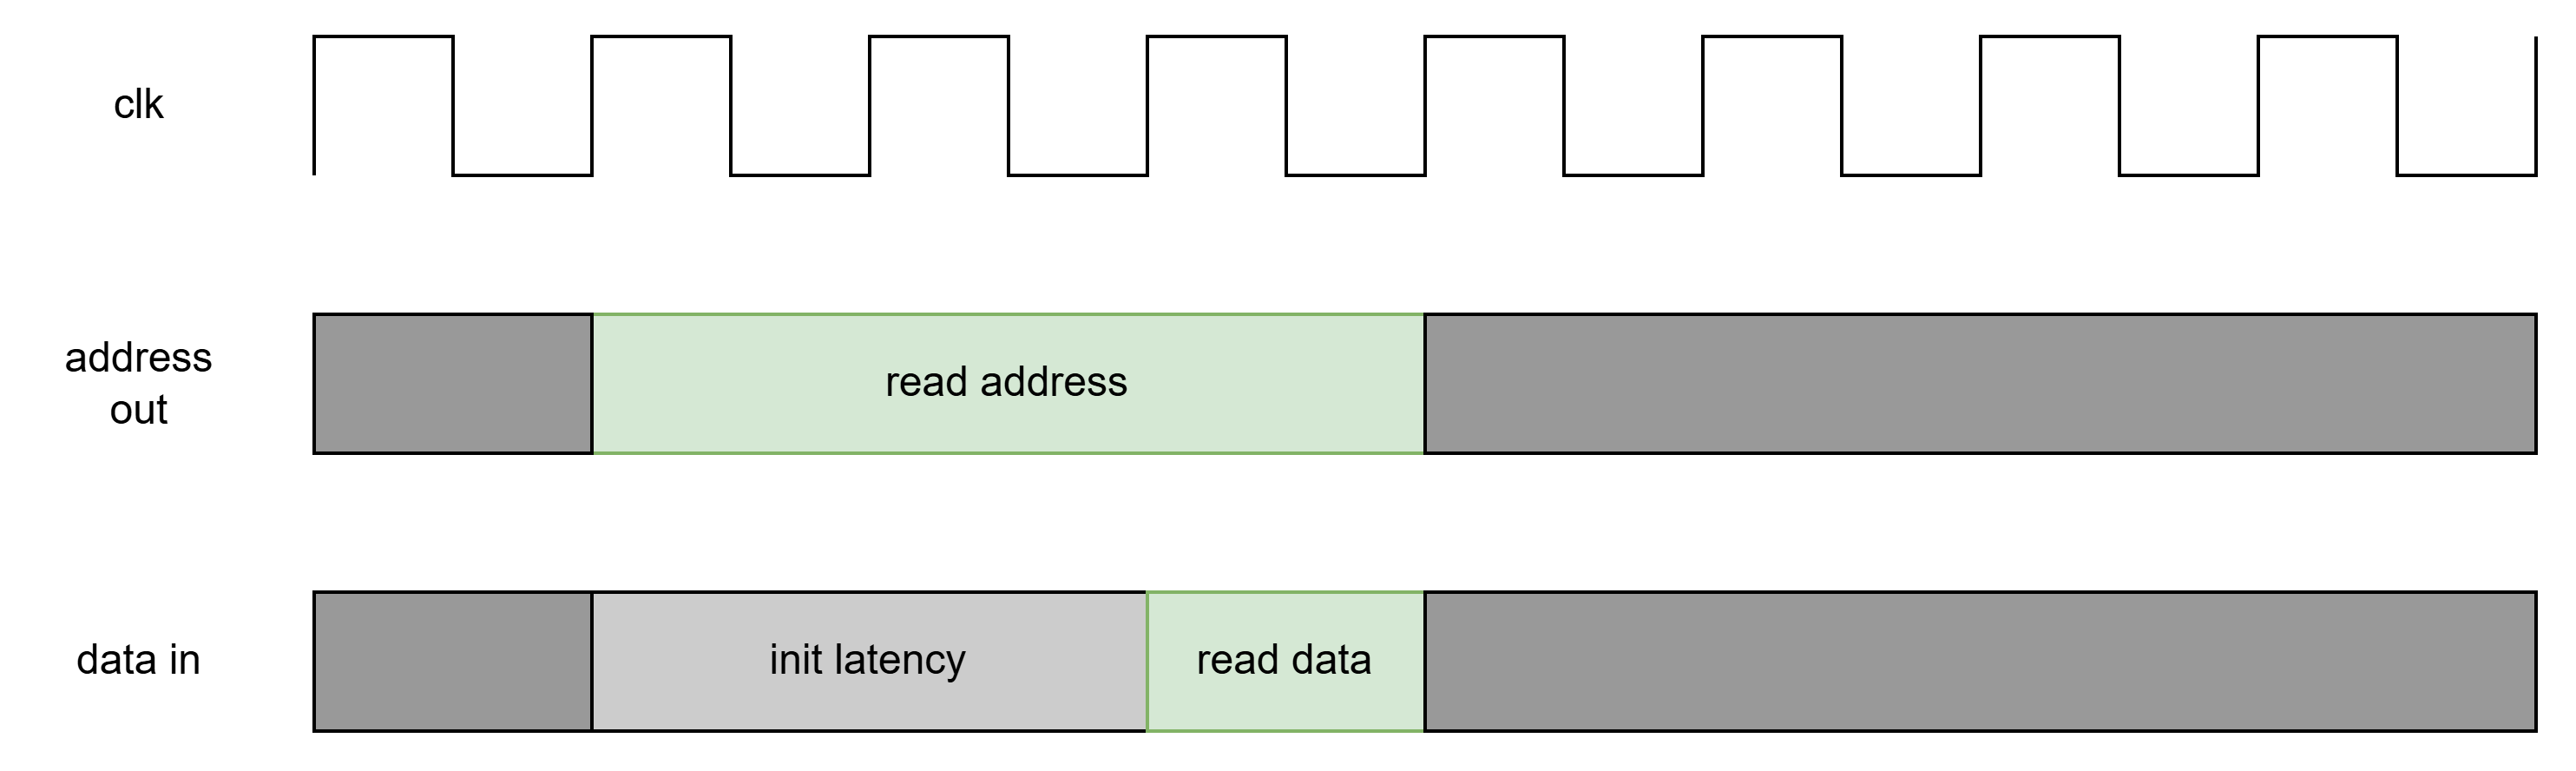
\includegraphics[width=\textwidth]{Figures/single_read.png}
\caption{Single access read operation \cite{Nolting2024Datasheet}.}
\label{fig:singleread}
\end{figure}

\begin{figure}[H]
\centering
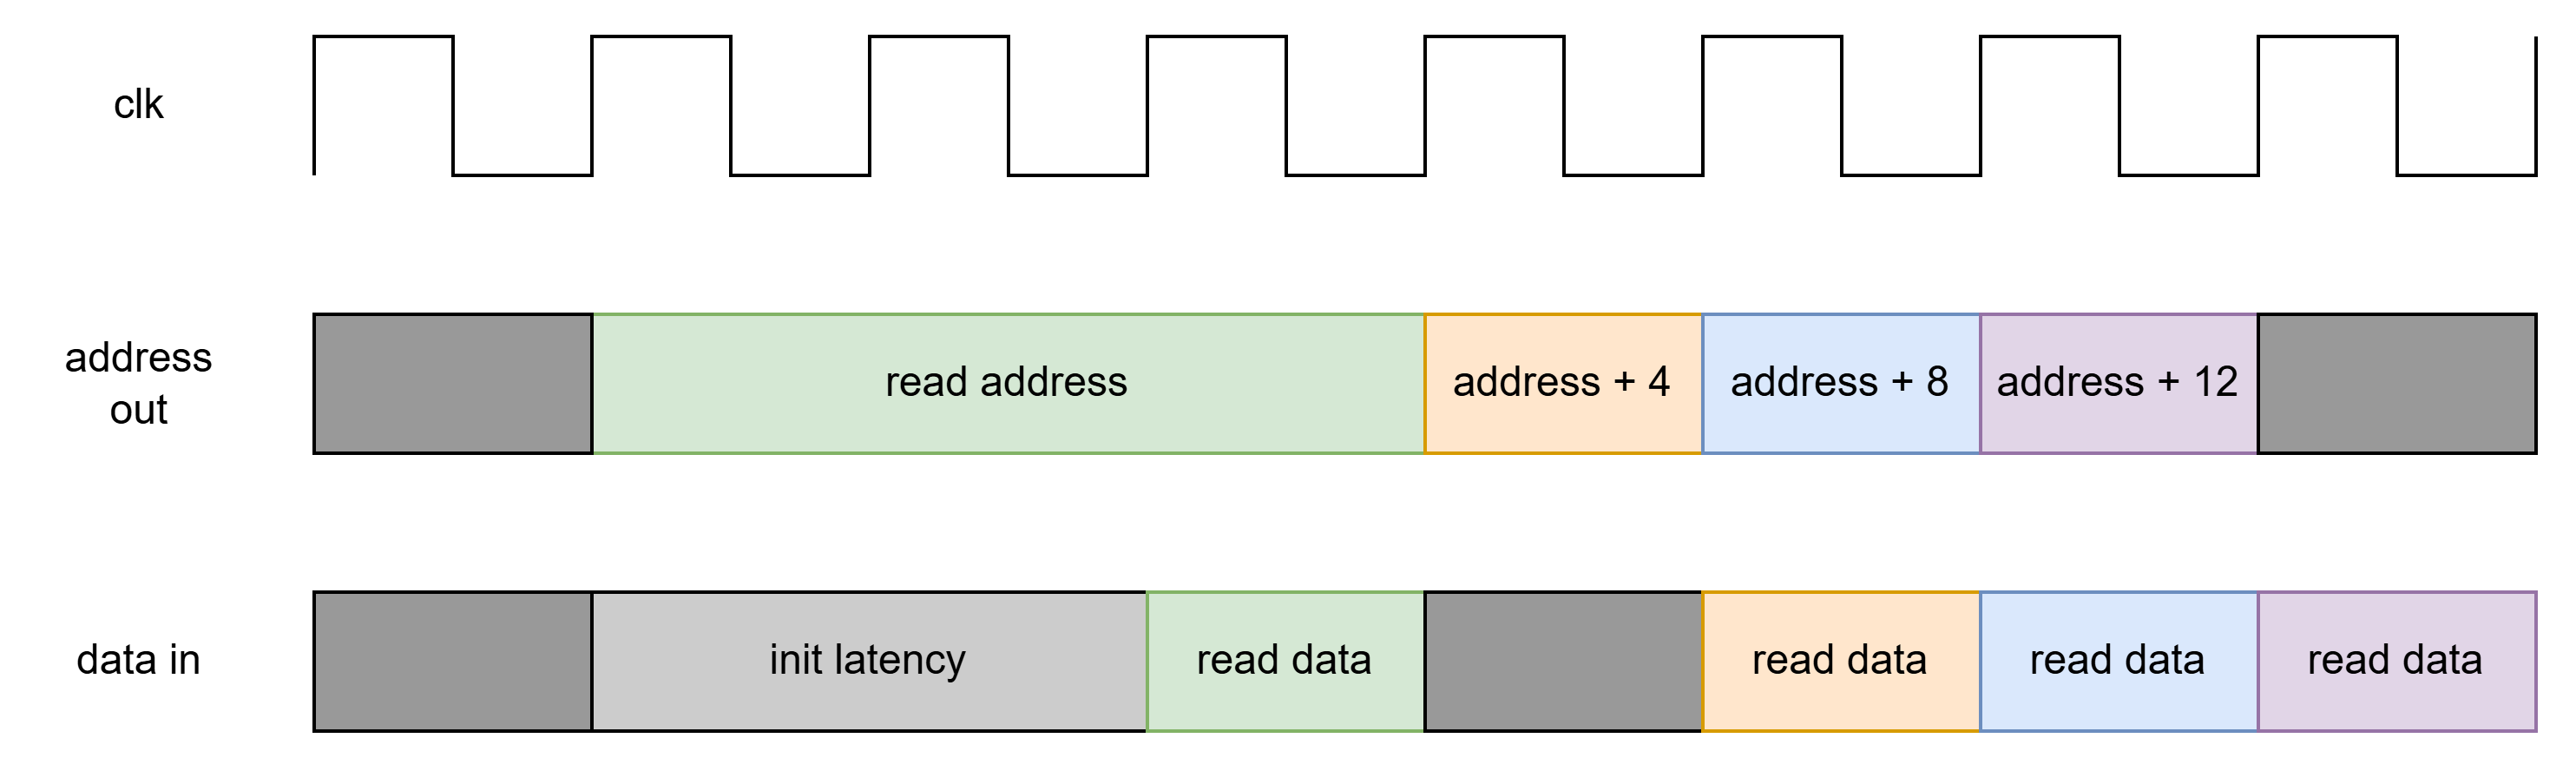
\includegraphics[width=\textwidth]{Figures/burst_read.png}
\caption{Burst read transfer \cite{Nolting2024Datasheet}.}
\label{fig:burstread}
\end{figure}


As explained in Section \ref{sec:per_chunk}, the per-chunk strategy accesses model data through a different strategy, however it is still by the same underlying cost as the per-class strategy. Here each mask word is read from DDR2 at the moment it is needed during evaluation, and the early exit terminates a clause after its first failing chunk. This leads to only part of the model being read for any given inference. Despite reading far less data than the per-class strategy, memory access is still the main bottleneck. This can be seen in Figure \ref{fig:chunk_vs_score_variance}, where the standard deviation $\sigma$ of the per-chunk inference time is 3.6 $\times$ higher than that of the per-class scoring time. As the difference between the two is that per-chunk inference reads the chunk words from DDR2, this points to the fact that the large difference in timing also stems from this.

It is worth noting that the per-chunk total is in fact lower than the per-class total by a factor of roughly 2.6, even though the per-class strategy was introduced to reduce DDR2 traffic. The per-class strategy forfeits the early exit, since it must copy every clause of a class into DMEM before any evaluation begins, and therefore moves the entire 4 MB model unconditionally on every inference. The per-chunk strategy moves only the portion of the model that the early exit does not skip. Neither strategy, however, escapes the fundamental cost of transporting the model out of DDR2. The per-chunk strategy pays it as scattered reads whose cost is dominated by access latency during evaluation, and the per-class strategy pays it as a single bulk preload dominated by transaction overhead. Both strategies are therefore memory-bound.


This result reframes the central question of the thesis. In the preceding project thesis \cite{JB2025}, the NoisyXOR model was small enough to reside entirely in on-chip DMEM, so no comparable data movement cost existed and clause evaluation was the dominant component of inference time. At that scale the workload was compute-bound, and accelerating clause evaluation through a custom instruction yielded a 4.42$\times$ speedup. At MNIST scale the model is roughly 8000$\times$ larger and cannot be held on-chip, which shifts the dominant cost from clause evaluation to memory transfer. The bottleneck is therefore not fixed by the algorithm but moves with the scale of the model, and at a realistic problem size it is the memory hierarchy, rather than the arithmetic, that limits performance. The implications of this shift for the effectiveness of the custom instructions are examined in the next section.